% Use the following line  only  if you're still using LaTeX 2.09.
%\documentstyle[icml2014,epsf,natbib]{article}
% If you rely on Latex2e packages, like most moden people use this:
\documentclass{article}
% use Times
\usepackage{times}
 % For figures
\usepackage{graphicx} % more modern
%\usepackage{epsfig} % less modern
\usepackage{subfigure} 
\usepackage{footnote}
\usepackage{amsfonts}
\usepackage{mdframed}

% For citations
\usepackage{natbib}
\usepackage{comment}
\usepackage{multirow}

\usepackage{float}

\floatstyle{plain} % optionally change the style of the new float
\newfloat{code}{H}{myc}

% For algorithms
\usepackage{algorithm}
\usepackage{algorithmic}
\usepackage{amsmath}
\usepackage{listings}

\lstset{language=Python,
  basicstyle=\ttfamily\footnotesize,
  keywordstyle=\color{blue}\ttfamily,
  stringstyle=\color{red}\ttfamily,
  commentstyle=\color{green}\ttfamily,
  aboveskip=0pt,
  belowskip=0pt,
  breaklines=true
}

\setlength{\abovedisplayskip}{0cm}
\setlength{\belowdisplayskip}{0cm}

\usepackage{mathtools}


\newcommand\myeq{\stackrel{\mathclap{\normalfont\mbox{{\tiny def}}}}{=}}


\usepackage[compact]{titlesec}
\titlespacing{\section}{0pt}{0.5ex}{0.3ex}
\titlespacing{\subsection}{0pt}{0.2ex}{0ex}
\titlespacing{\subsubsection}{0pt}{0.1ex}{0ex}

\newcommand{\startcompact}[1]{\par\vspace{-0.75em}\begin{#1}%
  \allowdisplaybreaks\ignorespaces}

\newcommand{\stopcompact}[1]{\end{#1}\ignorespaces}

\usepackage{paralist}

\makeatletter
\ifcase \@ptsize \relax% 10pt
  \newcommand{\miniscule}{\@setfontsize\miniscule{4}{5}}% \tiny: 5/6
\or% 11pt
  \newcommand{\miniscule}{\@setfontsize\miniscule{5}{6}}% \tiny: 6/7
\or% 12pt
  \newcommand{\miniscule}{\@setfontsize\miniscule{5}{6}}% \tiny: 6/7
\fi
\makeatother

\newcommand {\aplt} {\ {\raise-.5ex\hbox{$\buildrel<\over\sim$}}\ }

\newcommand{\eqn}[1]{Eqn.~\ref{eqn:#1}}
\newcommand{\fig}[1]{Fig.~\ref{fig:#1}}
\newcommand{\tab}[1]{Table~\ref{tab:#1}}
\newcommand{\secc}[1]{Section~\ref{sec:#1}}
\def\etal{{\textit{et~al.~}}}
\newcommand{\BigO}[1]{\ensuremath{\operatorname{O}\left(#1\right)}}
\usepackage[symbol*]{footmisc}

\DefineFNsymbolsTM{myfnsymbols}{% def. from footmisc.sty "bringhurst" symbols
  \textasteriskcentered *
  \textdagger    \dagger
  \textdaggerdbl \ddagger
  \textsection   \mathsection
  \textbardbl    \|%
  \textparagraph \mathparagraph
}%


% As of 2011, we use the hyperref package to produce hyperlinks in the
% resulting PDF.  If this breaks your system, please commend out the
% following usepackage line and replace \usepackage{icml2014} with
% \usepackage[nohyperref]{icml2014} above.
\usepackage{hyperref}

% Packages hyperref and algorithmic misbehave sometimes.  We can fix
% this with the following command.
\newcommand{\theHalgorithm}{\arabic{algorithm}}

% Employ the following version of the ``usepackage'' statement for
% submitting the draft version of the paper for review.  This will set
% the note in the first column to ``Under review.  Do not distribute.''
%\usepackage{icml2014} 
% Employ this version of the ``usepackage'' statement after the paper has
% been accepted, when creating the final version.  This will set the
% note in the first column to ``Proceedings of the...''
\usepackage[accepted]{icml2014}



\begin{document} 

\twocolumn[
\icmltitle{Learning to Reason\\{\small PhD Thesis Proposal}}

\icmlauthor{Wojciech Zaremba}{woj.zaremba@gmail.com}
\vskip +0.1in
\icmlauthor{Advisors:}{}
\vskip +0.03in
\icmlauthor{Rob Fergus}{fergus@cs.nyu.edu}
\vskip +0.03in
\icmlauthor{Yann LeCun}{yann@cs.nyu.edu}
\icmladdress{New York University}

\icmlkeywords{computer vision, convolutional neural networks, recurssive neural networks, natual language processing, recurrent neural networks, language model, LSTMs, program understanding, artificial intelligence}

\vskip 0.3in
]

\begin{abstract}

Neural networks proven to be a very powerful models for object recognition \cite{krizhevsky2012imagenet}, 
natural language processing \cite{mikolov2012statistical}, speech recognition \cite{graves2013speech}, and many others \cite{sutskever2014sequence}. 
However, there is still a huge gap between them, and an intelligent systems. 
I identify several potential unaddressed skills, which intelligent systems should possess: 
(1) reasoning abilities, (2) capability to integrate with external interfaces and (3) small sample complexity. My research focuses on tackling this problems. 

\end{abstract} 

\section{Introduction}
It's clear that by improving performance of current statistical learning systems, 
we won't be able to make them intelligent. Even if our object recognition system would yield
$0\%$ of prediction error, they wouldn't be intelligent. Same applies to speech 
recognition systems, machine translation and others. This work asks what skills are necessary for statistical
learning system to become ``intelligent''. Moreover, it attempts to address this remaining unaddressed skills. 


I believe, that crucial, poorly addressed skills that intelligent system has to poses are
(1) reasoning abilities, (2) capability to integrate with external interfaces and (3) small sample complexity. 
I would like to address all this problems within a seamless system. The same system should be used across
different tasks, and should be able to emulate simpler models. 


I have partially addressed some of proposed problems. I will make clear over the further part of this proposal, 
which parts have been addressed, and which are future goals.



\section{Reasoning abilities}

\textit{Reasoning} - ``the process of forming conclusions, judgments, or inferences from facts or 
premises''\footnote{Definition from \url{http://dictionary.reference.com/browse/reasoning}}.
\\
\\
System that can reason should be able to understand high level concepts like 
\begin{itemize}
 \item understand scope
 \item being able to memorize 
 \item branching
 \item repetitions
 \item and many more
\end{itemize}
Each of this skills could be solved in particular domain. However, such approach limits use of such system,
and assumes that we know a priori all possible scenarios. 
Moreover, I think that, intelligent reasoning system cannot be based only on predefined rules. 
Intelligent system has to be based on pattern matching, and application of learnt heuristic algorithms. 


There are many domains where we can test if our system can reason, and if it's able to learn postulated concepts. Eventually,
I would like to use the same tools for all domains. 
Domains of my interest are learning about computer programs, and 
proving mathematical theorems.
This domains are rich in scoping, branching, pattern repetition, and so on. Drawing
high level conclusions in such domains requires sophisticated reasoning skills.

\subsection{Reasoning in computer programs}
The first reasoning task that I am interest in is to train statistical models meaning of computer programs.
I propose one instance of program understanding.
Task is to take a program as an input (in our case character-by-character), and predict program evaluation. 
Prediction of program evaluation requires understanding every single operand of a program. For instance, in case of
addition it 
involves bit shifts, and memorization of operations on digits. Moreover, programs contain variable assignment, if-statements, and so on.
We were able partially to address postulated problem
\cite{zaremba2014execute}.
Figure \ref{fig:prog} shows
an exemplary program, target for such program, and prediction that we obtained with recurrent neural network.

\begin{figure}
  \begin{code}
  \begin{mdframed}
  {\bf Input:}
  \begin{lstlisting}
  f=(8794 if 8887<9713 else (3*8334))
  print((f+574))
  \end{lstlisting} 
  {\bf Target:} 9368. \\
  {\bf Model prediction:} 9368. 
  \end{mdframed}
  \end{code}
  \caption{An exemplary program that we take as an input. Task is to predict program evaluation. We have 
  achieved high performance on this task \cite{zaremba2014execute}.}
  \label{fig:prog}
\end{figure}


Current results are promising, however they are very limited. We are able to deal with programs
that can be evaluated by reading them once from left-to-right. Generic programs are not like that.
Our reasoning system has to be able to evaluate for arbitrary long time, if
task requires it. Moreover, it shouldn't be limited by finite memory size. Memory should be available
as an interface \ref{sec:interface}.


\subsection{Reasoning in mathematics}
It's known that theorem proving is an intractable task in computational sense. 
However, humans are able to prove theorems. They have to employ a prior
knowledge. They fit known mathematical ``tricks'' to the new problem.


More formally, we can think about proofs as a multiple axioms application that starts with
hypothesis that we want to prove. This way mathematical skills can be perceived as 
learning prior over trees of axioms. This prior ``suggests'' us which sequence of axioms is more
likely to lead to the theorem proof. 


My interest lies in learning such prior in some constrained mathematical 
domain. Our recent work \cite{zaremba2014learning}, concerns identities 
over polynomials over matrices. Figure \ref{fig:ident} shows \ref{fig:ident}


\begin{figure}
  \centering
  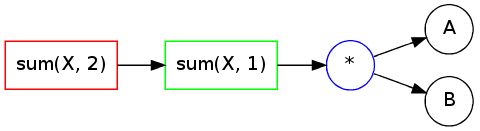
\includegraphics[width=0.48\textwidth]{imgs/example1_brute.png}\\
  {\bf Is equivalent to:}\\
  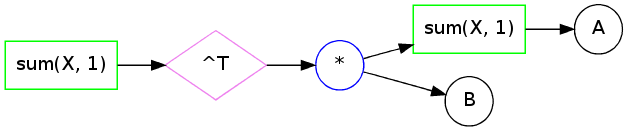
\includegraphics[width=0.48\textwidth]{imgs/example1_opt.png}\\
  \caption{\cite{zaremba2014learning}}
  \label{fig:ident}
\end{figure}


\section{Interface learning}
\label{sec:interface}
Contemporary machine learning systems are closed in a box.
They have limited access to the training dataset, 

, and cannot 
interact with external interfaces.


Initial advances in machine learning, where lead by engineering features, 
e.g histogram of colors, SIFT (Scale-invariant feature transform) features. 
This approach has its limitations, and its fragile. Moreover, it requires a 
human expert to train the system for the every new domain. Ideal system should 
have access to external interfaces that might give access to information, or simplify it processing. 
Interfaces that I have in mind are following (1) an external memory \cite{weston2014memory, graves2014neural}, 
(2) grid that helps to process images, (2) search engine, 
(4) Linux syscalls, or (5) execution environment like python interpreter. External interfaces are not-differentiable, 
and their state space is massive. This obstacles could potentially be addressed by learning a differentiable 
model that describes them (e.g. neural network). Neural network would simulate such 
external interface for purpose of being differentiable in a model-based reinforcement learning approach. 
This work is under progress.

\section{Small sample complexity}
Current deep learning systems suffer of large sample complexity. Such 
high sample complexity hinders potential use of the systems in online 
learning systems (e.g. robots). It’s expected that during the initial phase of 
learning any system without prior knowledge would need to consume a large number of samples. 
We hope that over the time of training, sample complexity should drop. However, this is 
not observed in current systems. I propose several approaches how sample complexity can be decreased. 
Meta-optimizer is a target solution. However, I propose some intermediate solutions, that can potentially help.

\subsection{Augmentation marginalization}

\subsection{One-shot learning objective}


This work is under progress.

\subsection{Meta-optimizer}
I would like to build a meta-optimizer that could 
overcome this limitation. Such optimizer would consume gradients of a neural network, 
and would decide on the next update step. Optimizer itself could be parameterized 
with a neural network. Proper weights could simulate any first order, gradient-based, 
learning algorithm like SGD, momentum, LBFGs etc. This implies that meta-optimizer 
subsumes all first order, gradient-based optimization techniques. Trained meta-optimizer 
could update the network in a much more clever way, and a single sample could provide enough knowledge.
This work is under progress.


\section{Discussion}
Tackling aforementioned problems would take us much closer to the
real intelligent systems, and defines for me the three main pillars 
of artificial intelligence. However, there are many other problems, which 
would need to be solved / integrated within such system to make it fully 
intelligent, e.g. navigation, learning by imitation, cooperation, and many others.
I hope that, all other skills can be integrated by means of external interface, and
don't have to be modelled in any special way. For instance, navigation skill could emerge 
as an use two interfaces (1) GPS location interface, and (2) an external memory.


\section{Disclaimer}
This is my personal opinion, and it shouldn't be judged in scientific way.


I strongly believe that creation of artificial intelligence is potentially
dangerous. However, I think, that more dangerous is avoiding to create it.
We exhaust resources of our planet in rapid fashion, and lack of resources 
leads to wars. The only way to have abundance of resources is to make them free.
Artificial intelligence could make all resources virtually free. The only remaining
question is if human can accept world where everything is given.


\bibliography{bibliography}
\bibliographystyle{icml2014}

\end{document} 

